\begin{titlepage}
  \begin{center}

  {\Huge PISO}

  \vspace{25mm}

  
\includegraphics[width=0.90\textwidth,height=\textheight,keepaspectratio]{img/AFRL.png}

  \vspace{25mm}

  \today

  \vspace{15mm}

  {\Large Jay Convertino}

  \end{center}
\end{titlepage}

\tableofcontents

\newpage

\section{Usage}

\subsection{Introduction}

\par
This core converts parallel input data into serial output data. This is done on a positive clock edge in relation to a active high enable. PISO is useful for many parallel to serial operations such as UARTS, SPI, i2c, 1553, etc. This is a fusesoc 2.X compatible core and its VLNV is AFRL:simple:piso:X.X.X.
\subsection{Dependencies}

\par
The following are the dependencies of the cores.

\begin{itemize}
  \item fusesoc 2.X
  \item iverilog (simulation)
  \item cocotb (simulation)
\end{itemize}

\subsection{In a Project}
\par
This core is designed to be used on the same clock domain as the input parallel data. The serial output rate is set by the enable.
The enable should only be pulsed for one clock cycle. If the clock is the rate the enable should be tied high. Load has to be
used to load the input data to the register and reset the output count. The data count provides other cores a bit count to know
what bit currently being output from the core. On load the data output is the previous bit till the enable is pulsed.
Once pulsed the output will be the data bit. Load will NOT change the output, also can be zeroed by just continuing to
se enable past the zeroth bit count (internal reg is filled with zeros).
The series of steps to use the core are as follows.
\begin{enumerate}
  \item Set pdata to input data, and set load to 1 (data will be loaded on positive clock edge to internal registers).
  \item Set load to 0 (dcount will now be the max number of bits in the word loaded).
  \item Pulse enable to 1 that is synced to the main clock. Only hold high for one period of the master clock.
  \item Data bit will be output on the serial line and held till next enable.
  \item Repeat enable pulse until dcount is equal to 0.
\end{enumerate}

Adding the core to a fusesoc project, outside of adding the verilog module to your code, requires the core be added as dependency.
Example:
\begin{lstlisting}[language=bash]
  dep:
    depend:
      - ">=AFRL:simple:piso:1.0.1"
\end{lstlisting}

Module instantiation:
\begin{lstlisting}[language=Verilog]
    piso #(
      .BUS_WIDTH(4)
    ) inst_piso (
      .clk(clk),
      .rstn(rstn),
      .ena(ena),
      .rev(rev),
      .load(load),
      .pdata(pdata),
      .reg_count_amount(reg_count_amount),
      .sdata(sdata),
      .dcount(dcount)
    );
\end{lstlisting}

\section{Architecture}
\par
This core is made to interface parallel to serial data. Data is loaded into the core, and then enable is pulsed to
push data out in a serial fashion. There is a count output that tells how many bits have been output. Data is only output
when the enable is toggled. The counter will start at the max number of bits UNLESS reg\_count\_amount is set to anything but 0.
For a 32 bit word this will be the decimal 32. If reg\_count\_amount is set it will start at that. Meaning bit sizes less than the bus
can be shifted out and properly terminated when 0 is reached. This will change the amount of data shifted in the internal register.
When toggled the counter will state the number of the bit present at the output. Starting at 32 means once enable is active,
and the counter is 31, bit 31 of the loaded word will now be output on the serial output. When the counter reaches 0 it means
the internal register has output all data since the last bit, 0, is now present on the serial output. Any further enable
pulses will not change the count but will shift the internal register. This will result in a 0 at the output since the register
shifts in 0 bits as each bit is output. All data is shifted in MSb to LSb or LSb to MSb. This is set with the rev input.
When active high (1) the LSb to MSb method is used. When rev is set to 0 MSb to LSb is used.
The only module is the piso module. It is listed below.

\begin{itemize}
  \item \textbf{piso} Convert parallel data to serial data. (see core for documentation).
\end{itemize}

Please see \ref{Module Documentation} for more information.

\subsection{Waveform}
\par
Below is a waveform in a typical application of the core for MSb to LSb. This shows the count up and how the enable is pulsed to decrement it.

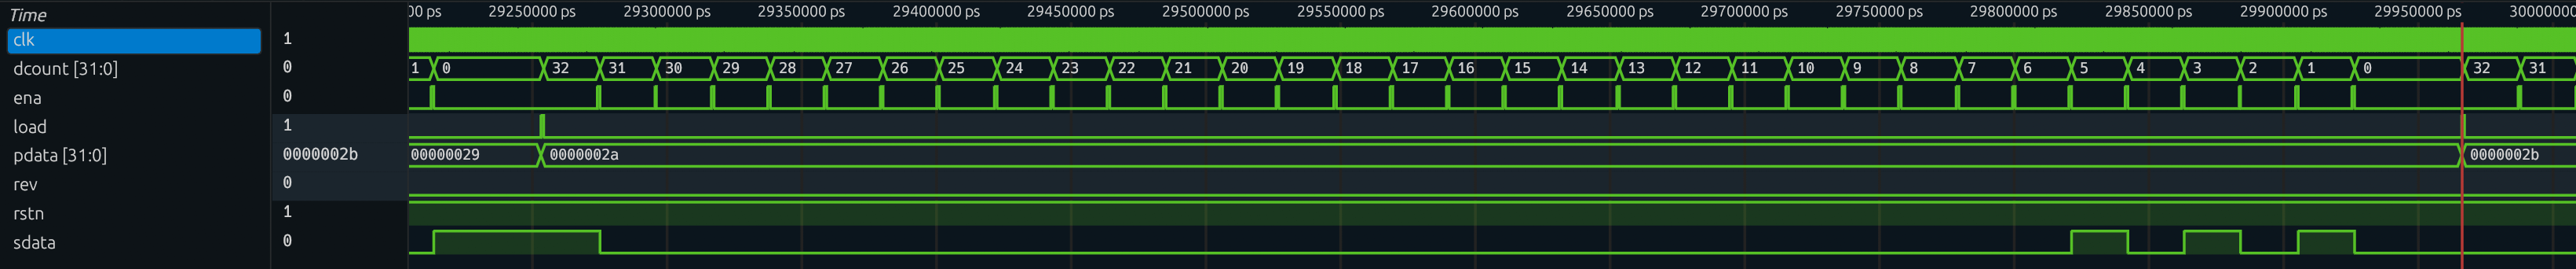
\includegraphics[width=\textwidth]{img/diagrams/waveform_rev0.png}

\par
Next shows the core with rev set to 1 for LSb to MSb operation.

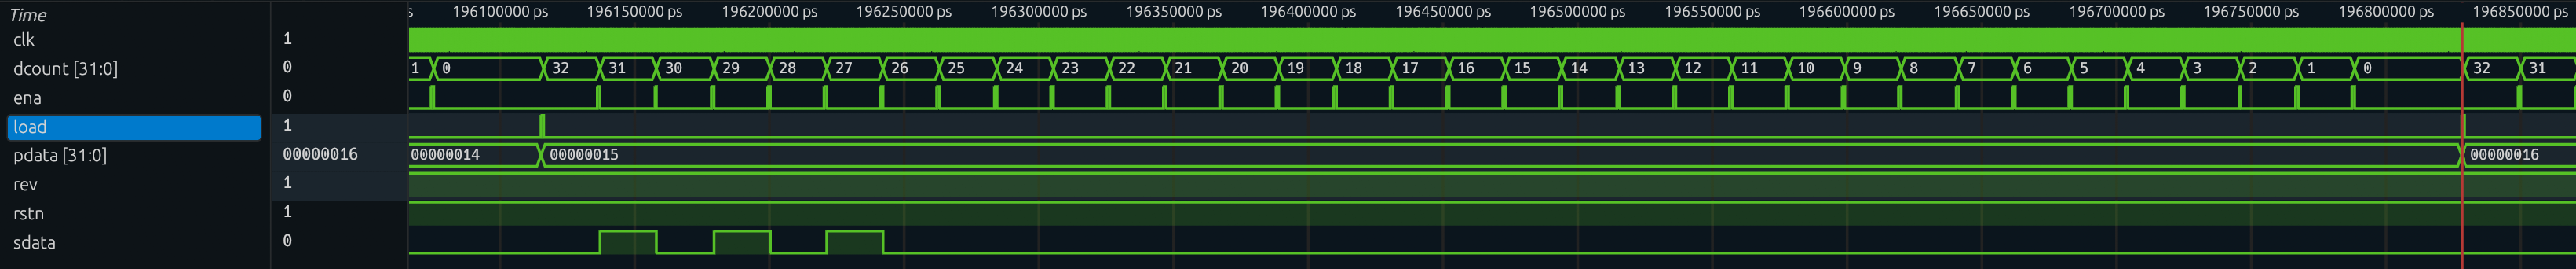
\includegraphics[width=\textwidth]{img/diagrams/waveform_rev1.png}

\section{Building}

\par
The PISO core is written in Verilog 2001. They should synthesize in any modern FPGA software. The core comes as a fusesoc packaged core and can be included in any other core as a dependency. Be sure you have meet the dependencies listed in the previous section. This core also has a target called lint for verilog linting useing verible-verilog-lint.

\subsection{fusesoc}
\par
Fusesoc is a system for building FPGA software without relying on the internal project management of the tool. Avoiding vendor lock in to Vivado or Quartus.
These cores, when included in a project, can be easily integrated into targets created based upon the end developer needs. The core by itself is not a part of
a system and should be integrated into a fusesoc based system. Simulations are setup to use fusesoc and are a part of its targets.

\subsection{Source Files}

\subsubsection{fusesoc\_info File List}
\begin{itemize}
\item src
	\begin{itemize}
	\item src/piso.v
	\end{itemize}
\item tb
	\begin{itemize}
	\item tb/tb\_piso.v
	\end{itemize}
\item tb\_cocotb
	\begin{itemize}
	\item {'tb/tb\_cocotb.py': {'file\_type': 'user', 'copyto': '.'}}
	\item {'tb/tb\_cocotb.v': {'file\_type': 'verilogSource'}}
	\end{itemize}
\end{itemize}


\subsection{Targets}

\subsubsection{fusesoc\_info Targets}
\begin{itemize}
\item default
	\begin{itemize}
	\item[$\space$] Info: Default for IP intergration.
	\end{itemize}
\item sim
	\begin{itemize}
	\item[$\space$] Info: Base simulation using icarus as default.
	\end{itemize}
\item sim\_cocotb
	\begin{itemize}
	\item[$\space$] Info: Cocotb unit tests
	\end{itemize}
\end{itemize}


\subsection{Directory Guide}

\par
Below highlights important folders from the root of the directory.

\begin{enumerate}
  \item \textbf{docs} Contains all documentation related to this project.
    \begin{itemize}
      \item \textbf{manual} Contains user manual and github page that are generated from the latex sources.
    \end{itemize}
  \item \textbf{src} Contains source files for the core
  \item \textbf{tb} Contains test bench files for iverilog and cocotb
    \begin{itemize}
      \item \textbf{cocotb} testbench files
    \end{itemize}
\end{enumerate}

\newpage

\section{Simulation}
\par
There are a few different simulations that can be run for this core. The backend used for testing is iverilog for verilog or cocotb simulations. Usually GTKWave is used to view the fst waveform output. Cocotb are the unit tests that attempt to give a pass/fail verification to the core operation.

\subsection{iverilog}
\par
iverilog is used for simple test benches for quick visual verification of the core. This will autofinish after it has
run up to a certain number of words have been output.

\subsection{cocotb}
\par
This method allows for quick writing of test benches that actually assert and check the state of the core.
These tests are much more conclusive since it will run all test vectors and generate a report if they
pass or fail. All tests output waves to a single fst file. The method of launching the tests is to use
fusesoc. These have not been written to use a python runner method or makefiles.
To use the cocotb tests you must install the following python libraries.
\begin{lstlisting}[language=bash]
  $ pip install cocotb
\end{lstlisting}

The targets available are listed below.
\begin{itemize}
  \item \textbf{sim\_cocotb} Standard simulation for PISO.
\end{itemize}

The targets above can be run with various parameters.
This test will check the input/output against each other to validate core operation.
\begin{lstlisting}[language=bash]
  $ fusesoc run --target sim_cocotb AFRL:simple:piso:1.0.1
\end{lstlisting}

\newpage

\section{Module Documentation} \label{Module Documentation}

\par

\begin{itemize}
\item \textbf{piso} PISO converter\\
\item \textbf{tb\_piso-v} Verilog test bench\\
\item \textbf{tb\_cocotb-py} Cocotb python test routines\\
\item \textbf{tb\_cocotb-v} Cocotb verilog test bench\\
\end{itemize}
The next sections document the module in detail.

